% don't remove the folling lines, and edit the defintion of \main if needed
\documentclass[../report.tex]{subfiles}
\providecommand{\main}{..}
\IfEq{\jobname}{\currfilebase}{\AtEndDocument{\biblio}}{}
\IfEq{\jobname}{\currfilebase}{%file for shortcuts

\newcommand{\nch}{\ensuremath{N_{\mathrm {ch}}\xspace}}
\newcommand{\Ncoll}{\ensuremath{N_{\mathrm {coll}}}}
\newcommand{\Npart}{\ensuremath{N_{\mathrm {part}}}}
\newcommand{\dNdeta}{\mathrm{d}N_\mathrm{ch}/\mathrm{d}\eta}
\newcommand{\snn}         {\ensuremath{\sqrt{s_{\mathrm {NN}}}}}
\newcommand{\kT}          {\ensuremath{k_{\mathrm {T}}}}

\newcommand{\pp}          {pp}
\newcommand{\pPb}         {pPb}
\newcommand{\pA}          {pA}
\newcommand{\PbPb}        {PbPb}
\newcommand{\AuAu}        {AuAu}
\newcommand{\CuCu}        {CuCu}
\newcommand{\pAu}         {pAu}
\newcommand{\dAu}         {dAu}
\newcommand{\lsim}        {\,{\buildrel < \over {_\sim}}\,}
\newcommand{\gsim}        {\,{\buildrel > \over {_\sim}}\,}
\newcommand{\co}[1]       {\relax}
\newcommand{\nl}          {\newline}
\newcommand{\el}          {\\\hline\\[-0.4cm]}}{}
% until here


\begin{document}
\section{High energy QCD with proton-nucleus collisions and ultra-peripheral collisions}

\textcolor{red}{Instructions/Comments}
\begin{itemize}
\item variable naming and unit conventions to be taken from review: https://arxiv.org/abs/0706.3356
\item please have a look at the .sty-files to check for symbols to be used
\item subsubsection may be omitted partially in final document, only working titles, please modify title if needed for your part, keep this structure for the moment to allow to separate different contributions more easily
\item luminosities to be used: PbPb: 13 nb$^{-1}$ @ 5.5 TeV ATLAS/CMS/ALICE, LHCb to be seen, about a factor 10 less,
pPb: 2000~nb$^{-1}$ @ 8.8 TeV for ATLAS/CMS, LHCb: 250~nb$^{-1}$@8.8~TeV for both orientation, 250~nb$^{-1}$ for ALICE @ 8.8 TeV for both configurations
\item please keep for the moment the 'headers' for the subparts
\item we should make an effort to stay within 20 pages, even if it is not easy
\end{itemize}

\subsection{Introduction}
\label{sec:smallxIntro}
Editor: Nestor Armesto \\

Proton-nucleus \cite{Salgado:2011wc} and ultraperipheral \cite{Baltz:2007kq} collisions offer the opportunity to study the behaviour of QCD at high energies and large partonic densities \cite{Kovchegov:2012mbw}. As the theory of the strong interaction, QCD is analytically well understood only in a perturbative regime of small coupling constant and where QCD radiation can be treated linearly, i.e. hadrons and nuclei are considered as dilute partonic objects. But non-linear effects are unavoidable in QCD, and they should eventually dominate at large densities to be achieved at high energies and for large nuclei. It was proposed long ago \cite{Gribov:1984tu,Mueller:1985wy} that at such large densities a resummation of powers of density times coupling constant is possible, resulting in a non-perturbative but weak coupling regime where parton densities saturate, and whose effective field theory incarnation is the Color Glass Condensate (CGC) \cite{Gelis:2010nm}. Particle production in pA collisions in the forward rapidity region is dominated by small$-x$ partons in the nucleus. Therefore, saturation effects are expected to be largest there. Furthermore, UPCs as a source of large fluxes of quasi-real photons, provide the opportunity to study the partonic structure of protons (in pp and pA) and nuclei (in pA and AA).

On the other hand, the structure of nucleons and nuclei, and the mechanism of particle production at small $x$, are key ingredients for our understanding of heavy-ion collisions and for the characterisation of the produced hot dense medium. For hard probes, the nuclear modification of standard collinear parton densities is one of the uncertainties in the extraction of medium characteristics. For soft and semihard observables, both the parton densities and the detailed transverse structure of nucleons and nuclei are crucial ingredients for their description, e.g. for the initial conditions for hydrodynamical evolution \cite{Liu:2015nwa,Weller:2017tsr,Mantysaari:2017cni}.

In the collinear framework, parton densities inside nuclei (nPDFs) \cite{armestodis2018} are poorly constrained due to two facts. On the one hand, data come from a large variety of nuclei and the number of data points for any of them, particularly for Pb for which it is less than 50 coming from fixed target DIS and DY experiments and from pPb collisions at the LHC, is very small compared to proton analysis. This fact makes the fit for a single nucleus impossible and the modeling of the $A$-dependence of the parameters in the initial conditions mandatory. On the other hand, the region covered by existing data is very small for the requirements of present hadronic colliders, see Fig. \ref{fig:smallx1}. In spite of the uncertainties (in the applicability of collinear factorisation, scale choices, etc.) for their extraction in hadronic collisions and UPCs, these are the only experimental systems where they can be constrained before electron-ion colliders become available. The most up to date analysis include between 1000 and 2000 data points for 14 nuclei and are performed at next-to-leading accuracy \cite{deFlorian:2011fp,Kovarik:2015cma,Eskola:2016oht} (even there exists some preliminary attempt at next-to-next-to-leading \cite{Khanpour:2016pph}). Differences between them mainly arise from the different sets of data included in the analysis and from the different functional forms employed for the initial conditions to be fitted. All in all, all parton species are very weakly constrained at small $x<10^{-2}$, gluons at large $x>0.2$, and flavour decomposition is largely unknown - a natural fact for $u$ and $d$ due to the approximate isospin symmetry in nuclei. The impact of presently available LHC data, studied in \cite{Eskola:2016oht}, is quite modest with some constrains on the gluon in the region $0.01<x<0.3$.

\begin{figure}[htb]
\centering
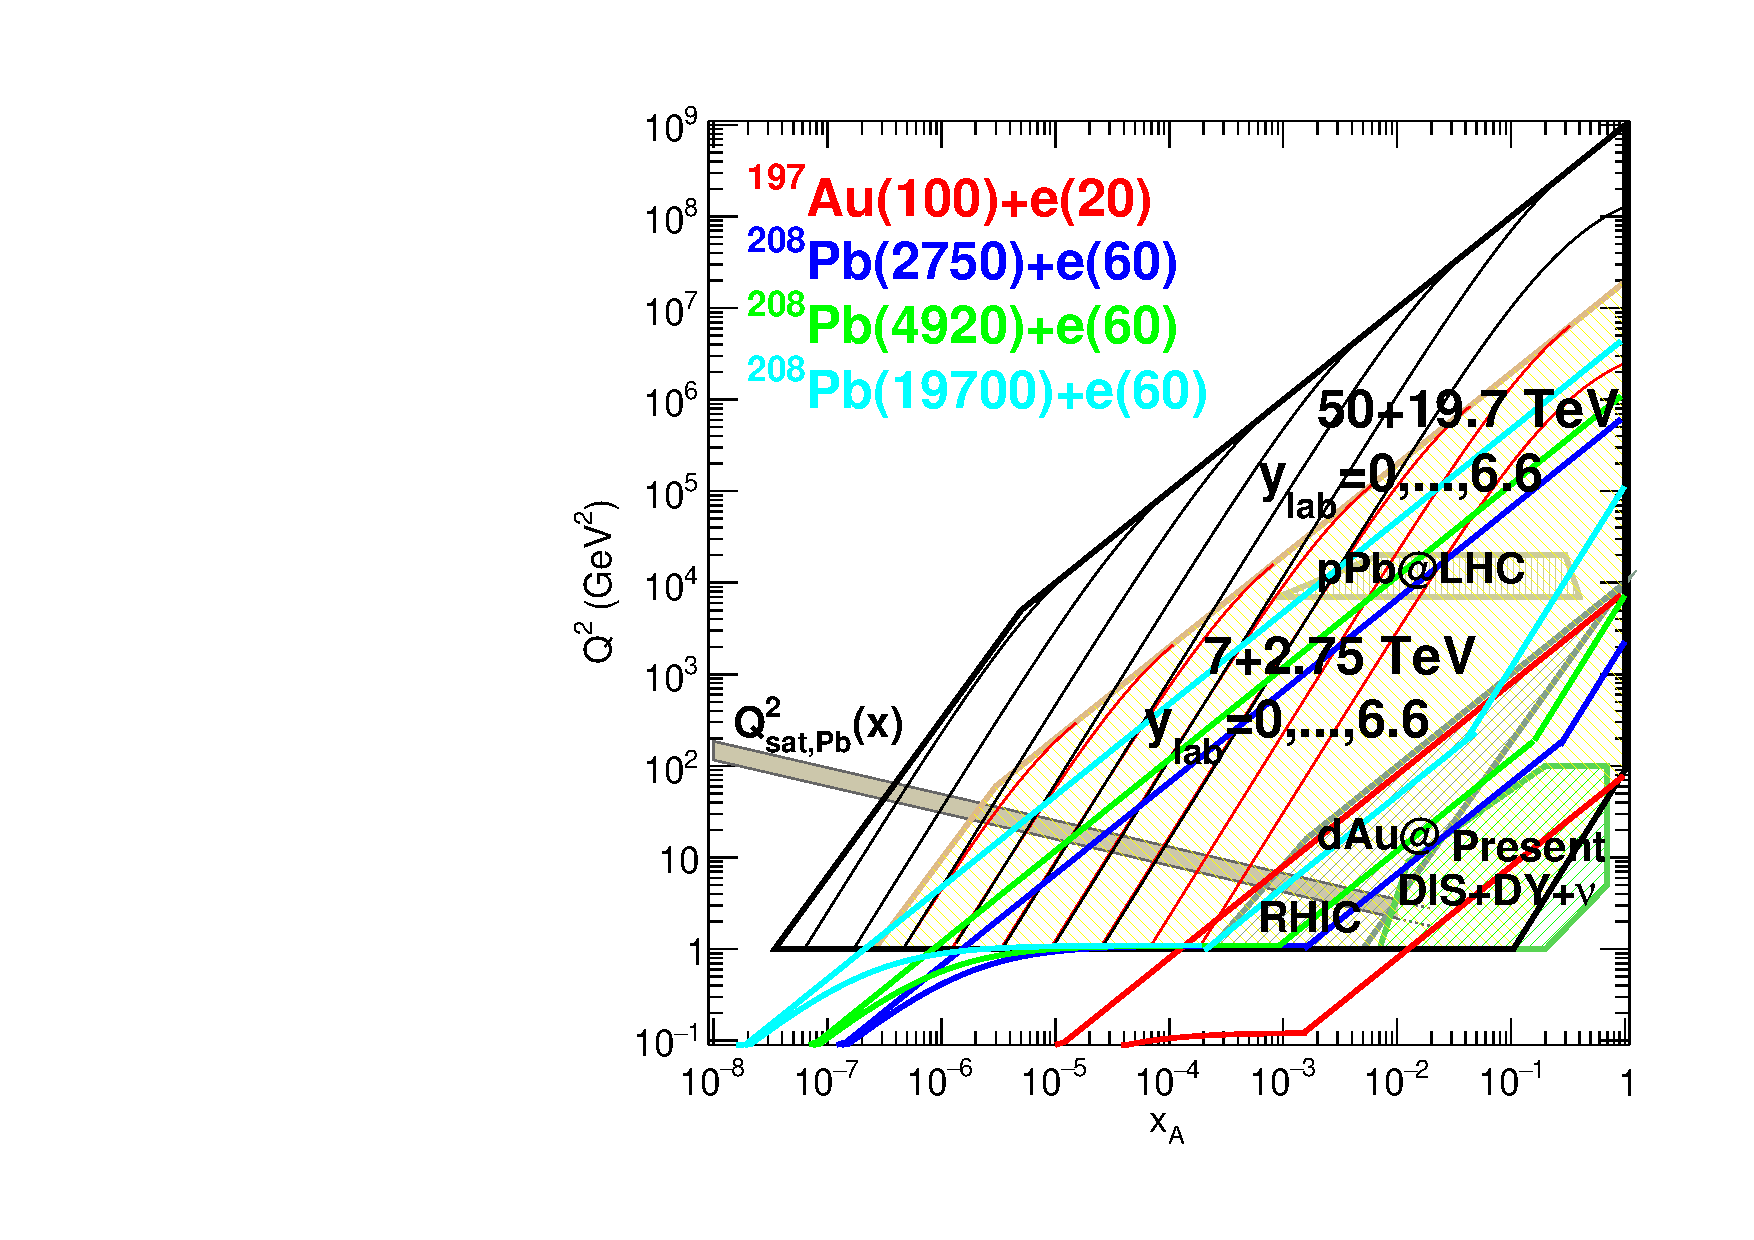
\includegraphics[width=0.45\textwidth]{\main/smallx/fig/FHC7_3.pdf} \hfill 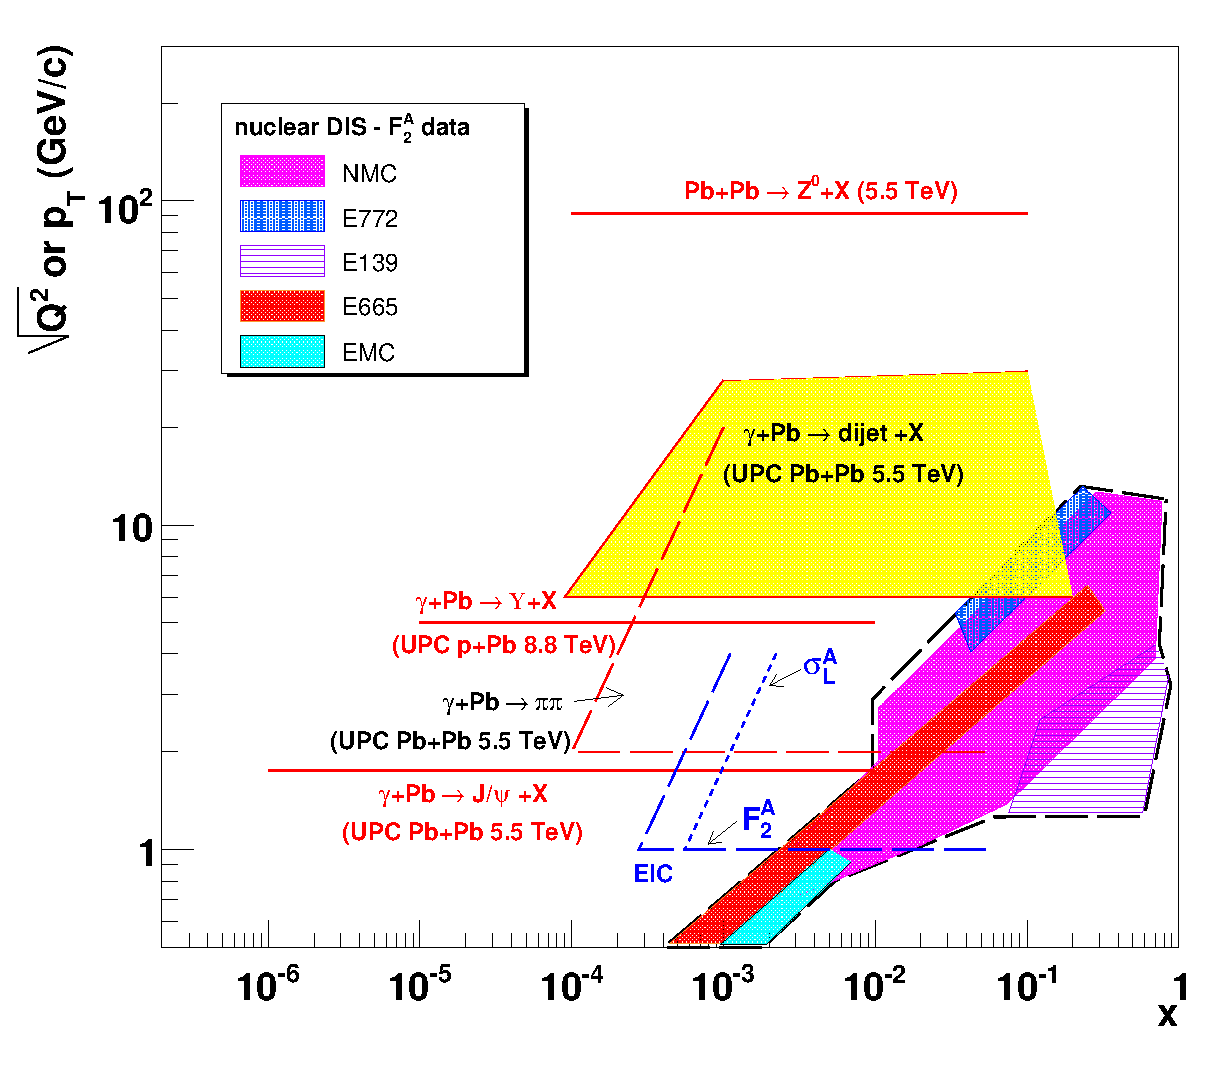
\includegraphics[width=0.45\textwidth]{\main/smallx/fig/upc_lhc_x_Q_map_5.eps}
\caption{Left: $x$-$Q^2$ plane to be explored in proton-nucleus at the LHC and the FCC, and in  proposed electron-nucleus colliders, compared with the regions where the experimental data presently used in the EPPS16 analysis \cite{Eskola:2016oht} lie. Right: $x$-$Q^2$ plane to be explored in UPCs, taken from \cite{Baltz:2007kq}.}
\label{fig:smallx1}
\end{figure}

On the other hand, there have been recent claims \cite{Ball:2017otu,Abdolmaleki:2018jln} that resummation of logarithms of $x$ may be required for a better description of DIS data from HERA at small $x$, and searches for long range azimuthal correlations are undergoing \cite{zeusichep2018}. But no conclusive evidence of saturation (i.e. of non-linear dynamics) has been found in hadronic collisions. While the CGC provides a calculational framework for several observables in pp, pA and AA, see e.g. the reviews \cite{Albacete:2013tpa,Lappi:2015jka}, like the ridge, back-to-back hadron correlations in the forward region, multiplicities and transverse momentum distributions,$\dots$,  the explanations are not unique or they involve non-perturbative modeling, or they are affected by large theoretical uncertainties and, for some of them, higher-order calculations are missing, or the data lie at the border of phase space where extracting clear conclusions is very delicate. Therefore, high-energy pA collisions and UPCs are the systems where data can offer clear evidences of non-linear effects at work.

In Fig. \ref{fig:smallx1} we show the kinematic regions covered by proton-nucleus collisions at the LHC and the FCC (left, \cite{Dainese:2016gch}) and UPCs at the LHC (right), compared with the regions where data currently used to constrain nPDFs lie. A huge enlargement is evident. With respect to the presently existing data at the LHC, HL-LHC offers new improved detectors and larger statistics for some observables like dijets or photon-jet correlations, and the HE-LHC would enlarge the kinematic plane in a region intermediate between the LHC and the FCC. On the other hand, electron-nucleus collisions \cite{AbelleiraFernandez:2012cc,Accardi:2012qut}, if they eventually happen in the 2030's, would be complementary, albeit in a more restricted kinematical region, by offering measurements in a cleaner experimental environment (no pileup, full kinematic reconstruction) and under better theoretical control as first-principle calculations are easier in DIS. The comparison between the kinematic regions covered by the LHC and FCC in pA mode, and the EIC \cite{Accardi:2012qut} and the LHeC \cite{AbelleiraFernandez:2012cc} (60 GeV electrons colliding with the HL-LHC, HE-LHC or FCC nuclear beams) is shown in Fig. \ref{fig:smallx1} right.


\subsection{The physics of ultra-peripheral collisions}
Editor: see sub-parts\\
Indicative length: 6 pages\\
Figures: to be discussed based on available experimental material, preference to full scale upgrade, should be balanced in terms of experiments as well as topics\\
Tables: one large overview table for observables
\subsubsection{Experimental overview}
Editors: Christoph Mayer(ALICE), Evgeny Krishen (ALICE), Daniel Tapia Takaki (CMS), Zvi Citron (ATLAS), Michael Winn (LHCb)
Indicative length: 2 pages\\
Content: observable overview table ordered by rate including back-of-envelope calculations for stat. error if nothing else available and explanations to instrumentation (one paragraph per experiment with suitable comparison with Run1/2), short mentioning of 'far beyond' observables in terms of luminosity in same collision system as default.

Table~\ref{tab:UPCExpRun12} summarizes the current status of UPC
measurements in LHC Runs 1 and 2 for all four experiments.

%LHCb paragraph draft MW
LHCb is well suited for exclusive production studies in ultra-peripheral collisions. In particular, its optimisation for flavour physics within its acceptance 2<eta<5 warrant an excellent resolution for typical momenta in quarkonium and heavy-flavour exclusive production as demonstrated in cite conf-note. Its particle identification capabilities allow to efficiently look for final states with charged muons, pions, Kaons and protons. Exclusive diphoton analysis as pioneered in ATLAS and CMS are also conceivable with lower ET-thresholds. The feasibility of inclusive gamma-induced measurements will require further studies. In Tab.~\ref{tab:UPCExpRun12} conceivable final states with suitable kinematic selections for analysis with LHCb are given.

%ALICE paragraph draft CM
In LHC runs 3 and 4 ALICE \cite{Abelevetal:2014cna} will take data in
both in triggered and in continuous readout mode,
\cite{Buncic:2015ari}. Using continuous
readout \cite{Antoniolietal:2013} essentially the full delivered luminosity can be integrated
because there is no loss of statistics due to trigger
inefficiencies. The acceptance for UPC events is significantly larger
than in LHC runs 1 and 2; it is determined by the tracking
efficiencies and the geometrical acceptances of the Inner Tracking
System (ITS) \cite{Abelevetal:2014dna}, of the TPC
\cite{ALICE:2014qrd} and of the Muon Forward Tracker (MFT) \cite{Uras:2012af}. Final
state neutron emission in UPC events can be detected by the
zero-degree calorimeters (ZDC) which will also take data in continuous
readout mode, and vetoes can be imposed using the fast interaction
trigger detector (FIT)
%and the forward diffractive detector (FDD)
.

\begin{table}[htbp]
  {\small
    \centering
    \begin{tabular}{|c|c|c|c|l|c|c|c|c|}
      \hline
      Exp. & Process & System & Ref. & Fiducial acceptance cuts \\
      \hline
          {\multirow{7}{*}{ALICE}} &
          $J/\psi \to ll$~$l=e,\mu$ &
          PbPb &
          \cite{Abbas:2013oua} &
          $|\eta_l|$~$<$~$0.9$,
          one of $p_{T,l}$~$>$~1~GeV/$c$
          %%, $|y|<0.9$
          \\
          &
          $\psi(2S)\to ll+\pi\pi$,~$l=e,\mu$ & %% (J/\psi)
          PbPb     &
          \cite{Adam:2015sia} &
          $|\eta_l|$~$<$~$0.9$,
          one of $p_{T,l}$~$>$~1~GeV/$c$
          %%,$|y|<0.9$
          \\
          &
          $\gamma\gamma\to ee$        &
          PbPb     &
          \cite{Abbas:2013oua}   &
          $|\eta_e|<0.9$,
          $m(ee)$~$\in$~$[2.2,2.6]$,~$[3.7,10]$~GeV/$c^2$
          \\
          &
          $\rho \to \pi\pi$           &
          PbPb     &
          \cite{Adam:2015gsa} &
          $|y(\pi\pi)|$~$<$~$0.5$
          \\
          &
          $J/\psi \to \mu\mu$         &
          pPb      &
          \cite{TheALICE:2014dwa}  &
          $2.5$~$<$~$|\eta|$~$<4.0$,
          $p_{T,\mu}$~$\gtrapprox$~$1$~GeV/$c$
          %,$2.5$~$<$~$y$~$<$~$4.0$
          \\
          &
          $J/\psi \to \mu\mu$ (peripheral)        &
          PbPb     &
          \cite{Abelev:2012ba}  &
          $3.7$~$<$~$|\eta|$~$<$~$2.5$,
          $p_{T,\mu}$~$\gtrapprox$~$1$~GeV/$c$
          %,$2.6$~$<$~$y$~$<$~$3.6$
          \\
          &
          $J/\psi \to \mu\mu$         &
          PbPb&
          \cite{Adam:2015gba} &
          $2.5$~$<$~$|\eta|$~$<4.0$,
          $p_{T,\mu}$~$\gtrapprox$~$1$~GeV/$c$
          %,$2.5$~$<$~$y$~$<$~$4.0$
          \\
          \hline
          CMS          &
          $J/\psi \to \mu\mu$         &
          PbPb     &
          \cite{Khachatryan:2016qhq}                  &
          $1.2$~$<$~$|\eta|$~$<$~$2.4$,
          $p_{T}$~$\in$~$[1.2,1.8]$~GeV/$c$,
          $1.8$~$<$~$|y|$~$<$~$2.3$
          \\
          \hline
          LHCb         &
          $J/\psi,\psi(2S) \to \mu\mu$&
          pp       &
          \cite{Aaij:2014iea}
          &
          $2.0$~$<$~$\eta$~$<$~$4.5$,~
          $p_T$~$>$~$0.4$~GeV/$c$,~
          $2.0$~$<$~$y$~$<$~$4.5$
          \\
          \hline
              {\multirow{2}{*}{ATLAS}} &
              $\gamma\gamma\to \mu^+\mu^-$ &
              {\multirow{2}{*}{PbPb}} &
              {\multirow{2}{*}{\cite{ATLAS:2016vdy}}} &
              $|\eta|$~$<$~$2.4$,
              $p_T$~$>$~$4$~GeV/$c$,
              $m$~$>$~10~GeV/$c^2$
              \\
              &
              dijet &
              &
              &
              $|\eta|$~$<$~$4.9$,
              sum-$E_T$~$>$~$5$
              \\
              \hline
    \end{tabular}
    \caption{Acceptances and observables: \textcolor{red}{MW: to be completed by experimental contacts, final layout and what in table to be decided, e.g. Ref. can be directly at experiment name for existing measurements and projections. The $p_T$-track selections for ATLAS,ALICE,CMS,LHCb represent not the limits of the reconstructibility but fiducial acceptance cuts that were chosen for those specific observables.}  }
    \label{tab:UPCExpRun12}
  }
\end{table}


In table~\ref{tab:ALICERun34Proj} the expected yields for heavy
quarkonia are shown, assuming an integrated luminosity of
13~nb$^{-1}$. In addition to heavy quarkonia there will be the
possibility to study $\rho$ and $\phi$ photoproduction via dimuon
decays at forward rapidity.

\begin{table}[htbp]
  {%%\tiny
    \centering
    \begin{tabular}{|c|c|c|c|}
      \hline
      Meson & $-4$~$<$~$y$~$<$~$-2.5$ & $-2.5$~$<$~$y$~$<$~$-1$ & $|y|$~$<$~$1$\\\hline
      J/$\psi$         & 580k   & 480k   & 3270k   \\
      $\Psi(2$S$)$     &  15.7k &  13.7k &   93.8k \\
      $\Upsilon(1$S$)$ & 760    & 900    & 7000    \\
      \hline
    \end{tabular}
    \caption{Expected yields for heavy quarkonia in central, forward and semi-forward configurations in ALICE
      assuming an integrated luminosity of 13~nb$^{-1}$.} \label{tab:ALICERun34Proj}
  }
\end{table}

\begin{table}[htbp]
 {%%\tiny
\centering
\begin{tabular}{|c|c|c|c|l|c|c|c|c|}
\hline
Experiment & published & systems & Ref. & kin.~constraints \\
\hline
\hline
&
$J/\psi \to l^+l^-$                    &
&
&
&
&
multi-diff., b-slope 
\\
&
Upsilon $\to l^+l^-$                   &
&
&
&
&
\\
&
$\psi(3S) \to D\bar{D}$                 &
&
&
&
&
\\
&
coherent $\phi \to$KK             &
&
&
&
&
\\
\hline
&
future $\gamma-\gamma$                 &
&
&
&
&
\\
\hline
&
$\eta_c$, ($\chi_{c0},\chi_{c2}$)    &
&
&
&
&
\\
&
4 $l$: 2$\times$Vector-meson   &
&
&
&
&
\\
&
$p\bar{p}$ ($\eta_c$)                 &
&
&
&
&
\\

\hline
\end{tabular}
\caption{Acceptances and observables: \textcolor{red}{CM: This is the second half of table 1 which I left in the document for now.}  }
}
\end{table}


\subsubsection{Detailed projections}
space for detailed projection studies; \\
one projection from ATLAS on dimuon invariant mass distribution from gamma-gamma, \\ MW: could be used as reference for rest of chapter: understand gamma-flux and can be used for luminosity measurement eventually

Vector meson cross section in Pb-Pb UPC can be expressed as a sum of two terms reflecting the fact that either of the colliding ions can serve as a photon source:
\begin{equation}
\sigma(y) = n(+y) \sigma_{\rm \gamma Pb}(+y) + n(-y) \sigma_{\rm \gamma Pb}(-y)
\end{equation}
The photoproduction cross sections $\sigma_{\rm \gamma Pb}(y)$ and $\sigma_{\rm \gamma Pb}(-y)$ are coupled and cannot be extracted unambiguously from the measured rapidity differential cross section. However one can decouple them by measuring vector meson production in UPC with and without additional neutron activity in Zero Degree Calorimeters. Measurement of $\sigma_{\rm 0N0N}(y)$ (no neutrons on both sides) and $\sigma_{\rm 0NXN}(y)$ (at least one neutron on one of the sides) cross sections provides a system of two equations of two unknown photoproduction cross sections $\sigma_{\rm \gamma Pb}(\pm y)$:
\begin{eqnarray}
\sigma_{\rm 0N0N}(y) &=& n_{\rm 0N0N}(+y) \sigma_{\rm \gamma Pb}(+y) + n_{\rm 0N0N}(-y) \sigma_{\rm \gamma Pb}(-y), \\
\sigma_{\rm 0NXN}(y) &=& n_{\rm 0NXN}(+y) \sigma_{\rm \gamma Pb}(+y) + n_{\rm 0NXN}(-y) \sigma_{\rm \gamma Pb}(-y),
\end{eqnarray}
where $n_{\rm 0N0N}(\pm y)$ and $n_{\rm 0NXN}(\pm y)$ are corresponding photon fluxes, calculable with high accuracy.

Solutions of this system of equations can be used to extract gluon shadowing at different scales under assumption that coherent photoproduction cross section is proportional to the squared gluon density at $Q = m_{V}/2$. For that  one can construct the nuclear suppression factor expressed as root square of the ratio of photoproduction cross section measured in Pb-Pb UPC and photoproduction cross section in the Impulse Approximation calculated as a reference photoproduction cross section off proton scaled by the integral over squared Pb form factor~\cite{Guzey:2013xba}:
\begin{equation}
S (x) = \left(\frac{\sigma_{\rm \gamma Pb}(x)}{\sigma_{\rm IA}(x)}\right)^{1/2}, \qquad {\rm where}\qquad x  = \frac{m_{V}}{\sqrt{s_{NN}}}\exp(-y).
\end{equation}
Resulting projections for the nuclear suppression factor are shown in fig.~\ref{fig:r} at different scales corresponding to $J/\psi$, $\psi(2S)$ and $\Upsilon(1S)$ photoproduction measurements. Uncertainties on luminosity (4\%), reference cross section (5\%) and photon flux (5\%) result in $\sim8$\% systematic uncertainty on the ratio $\sigma_{\rm \gamma Pb}(x)/\sigma_{\rm IA}(x)$ and $\sim 4$\% uncertainty on the nuclear suppression factor $S (x)$.

\begin{figure}
\centering
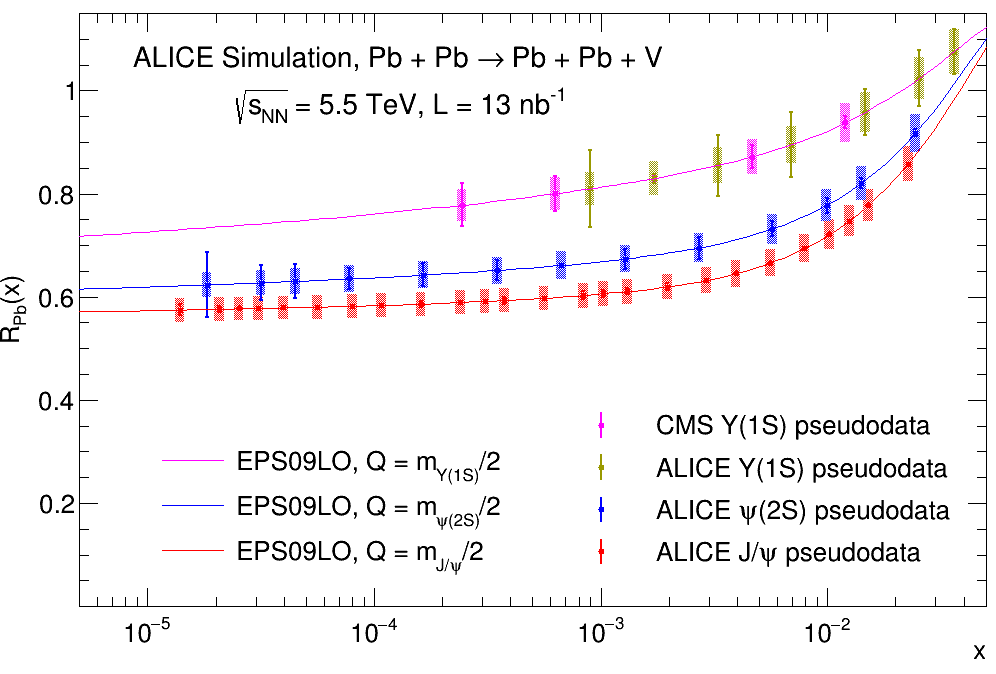
\includegraphics[width=0.6\textwidth]{\main/smallx/fig/suppression_factor.png}
\caption{Projections for gluon shadowing factor measured with heavy vector photoproduction in Pb-Pb UPC collisions at different scales.}
\label{fig:r}
\end{figure}

\subsubsection{Inclusive and diffractive dijet production in UPC}
Editors: Mark Strikman, Vadim Guzey + Aaron Angerami, Adrian Dimitru, Vladimir Skokov\\
Indicative length: 1-2 pages

Figures: Feynman graphs for jets in UPCs; 2 plots for $x_A$ dijet distributions in the inclusive
and diffractive cases.
\begin{itemize}
\item Introduction: inclusive and diffractive jets in UPCs (graphs)
\item jets in UPCs as novel probes of nuclear usual and diffractive PDFs
\item small-x nuclear diffractive PDFs
\item Status of collinear NLO formalism for inclusive and diffractive jet photoproduction;
lessons from HERA
Theoretical predictions for dijet distributions using NL0 pQCD + EPPS16, nCTEQ15, LTA nPDFs; conclusion about the magnitude of nuclear effects\end{itemize}

\subsubsection{Vector meson production}
Editors: Mark Strikman and Vadim Guzey + Jesus Guillermo Contreras Nuno + Spencer Klein\\
Indicative length: 1-2 pages

Figures: Feynman graph of incoherent VM photoproduction in UPCs; two-panel figure for the t-dependence for light and heavy VMs.
\begin{itemize}
\item Introduction: incoherent VM photoproduction in UPCs and nuclear shadowing, relation to
geometric fluctuations of the projectile and target
\item incoherent vs. coherent VM photoproduction from
point of view of accessing small-$x$, UPCs with e.m. nucleus excitation and forward neutron emission
\item Overview of the literature; general features vs. model-dependence;
comparison to existing LHC data
\item Predictions for run 2.
\end{itemize}

\subsubsection{Exclusive open charm production}
Author: Spencer Klein\\
Indicative length: 0.5-1 page


\subsection{The physics of pPb collisions}
Editors: see subparts\\
Indicative length 6-7 pages\\
Figures: to be discussed based on available experimental material, preference to full scale upgrade, should be balanced in terms of experiments as well as topics\\
Tables: one large overview table for observables
\subsubsection{Experimental overview}
Editors: Yen-Jie Lee (CMS), Marco van Leeuwen (ALICE), Zvi Citron (ATLAS), Michael Winn (LHCb)\\
Indicative length: 1-2 pages\\
Content: observable overview table ordered by rate including back-of-envelope calculations for stat. error if nothing else available and explanations to instrumentation (one paragraph per experiment with suitable comparison with Run1/2), short mentioning of 'far beyond' observables in terms of luminosity in same collision system as default.

%LHCb draft, try to be more explicit for new observables
In LHCb during Run 3 and 4, the average multiplicity in pPb and Pbp collisions will be smaller or very similar to the nominal conditions in pp running with an average  pile-up of visible pp interaction of around 5 collisions at improved performances. The low rates in pPb collisions allow to process the full inelastic rate in the HLT as already in Run 2. The software trigger system will allow to study pPb collisions with looser selections as in standard pp collisions. Hence, LHCb can fully profit from the luminosity increase including 0-pt heavy-flavour.  A natural focus for LHCb in pPb collisions is the study of heavy-flavour with improved statistical precision and, as a consequence of strongly increased control samples for tracking efficiency and particle identification, improved systematic uncertainties including fully reconstructed D and B-mesons as well Lc and Lb baryons. A new focus of LHCb, profitting from the increased luminosity, is the study of W,Z and in particular Drell-Yan down to low masses production at forward rapidity. For Drell-Yan, production, the vertex locator allows for a strong suppression of heavy-flavour decay muons. Direct photon studies in particular in the conversion channel will greatly profit from the increased luminosity. In Tab., we summarise conceivable final states with suitable kinematic selections profitting to a large extent from the pp experience.

% ALICE general first draft MvL
During run 3 and/or 4, ALICE will measure heavy flavor and charged particle production at mid-rapidity in pPb (and Pbp) collisions. These measurements will constrain the parton densities in the nucleus at moderate $x$. At forward and backward rapidity, measurements of W and Z production, as well as a range of quarkonia ($\PJgy$, $\PGyP{2}$, and the $\PGU$ family) will be performed. In particular the W and Z boson measurements will constrain the nuclear PDFs, while the quarkonia are also sensitive to final state effects.

% CMS draft EC
Using the larger pPb dataset available during Runs~3 and/or 4, CMS will further improve the precision on differential measurements of W and Z bosons (constraining quark and antiquark nPDFs), as well as dijet and ttbar production (gluon nPDFs). While first Run~2 results on W boson production already feature experimental uncertainties smaller than the nPDF ones, the larger luminosity by a factor 5 to 10 expected in Runs~3--4 will allow for another large jump in the constraints on nPDFs from data. In addition, novel studies will become possible, such as the measurement of differential ttbar distributions (CMS projection expected soon), for an improved constraining power on nPDFs, as well as the mass dependence of Drell-Yan production down to the $\PGU$ meson mass region. Heavy flavour meson cross sections will also be measured, which are sensitive to low-$x$ gluon nPDFs: D mesons ($\pt>0.5$\,GeV), B mesons ($\pt>5$\,GeV), prompt and nonprompt $\PJgy$ ($\pt>3$\,GeV), and $\PGUP{n}$ down to $\pt=0$.

\begin{table}[htbp]
 {\footnotesize
\centering
\begin{tabular}{|c|c|c|c|c|c|}
\hline
Experiment   & Observable & $p_{T}$[GeV/$c$]-range, mass & $y_{lab}$               & raw yield & physics interest \\
\hline
ALICE  & Z                &          & [-4.2,-3] [2,3.5] & uncertainty 3-4\%  (syst)  & nPDF       \\
       & W                &          & [-4.4,-3] [2,3.5] & unc 6-8\% (syst) & nPDF
\\
       &                  &          &        &                    &
\\
\hline
ATLAS  &                  &          &        &                     &        \\
       &                  &          &        &                    &
\\
       &                  &          &        &                    &
\\
\hline
CMS    &                  &          &        &                    &         \\
       &                  &          &        &                    &
\\
       &                  &          &        &                    &
\\
\hline
LHCb   &                  &          &         &                    &         \\

       &  $D\bar{D}$-correlations     &          &        &                    & TMD, saturation, collective behaviour  \\
       &  open-charm production     &          &        &                    & nPDF, factorisation breaking \\
 &  open-beauty production     &          &        &                    & nPDF, factorisation breaking \\
&  photons     &          &        &                    & nPDF, saturation \\
&  low-mass Drell-Yan   &          &        &                    & nPDF, saturation
\\
&  W-production     &          &        &                    & nPDF \\
&  Z-production     &          &        &                    & nPDF
\\
\hline
\end{tabular}
\caption{Acceptances and observables.  }
}
\end{table}

\subsubsection{Forward calorimeter upgrade of ALICE}
Author: Marco van Leeuwen
1 page

\subsubsection{Detailed projections}
Editors: experimental contacts from overview unless other contact given, description as short as possible with reference to publicly available material \\
Indicative length: 2 pages \\
Content: W,Z(ATLAS/CMS), Drell-Yan(CMS/ATLAS), dijet(CMS/ATLAS)\\
top (CMS/ATLAS), plot will be shown in extra part by David and Hannu \\
W,Z,low-mass Drell-Yan (LHCb), gamma (ALICE) \\
MW proposal plots: Dijets by CMS; W,Z by ATLAS/CMS (one triple differential from ATLAS)\\
\begin{figure}[htb]
\centering
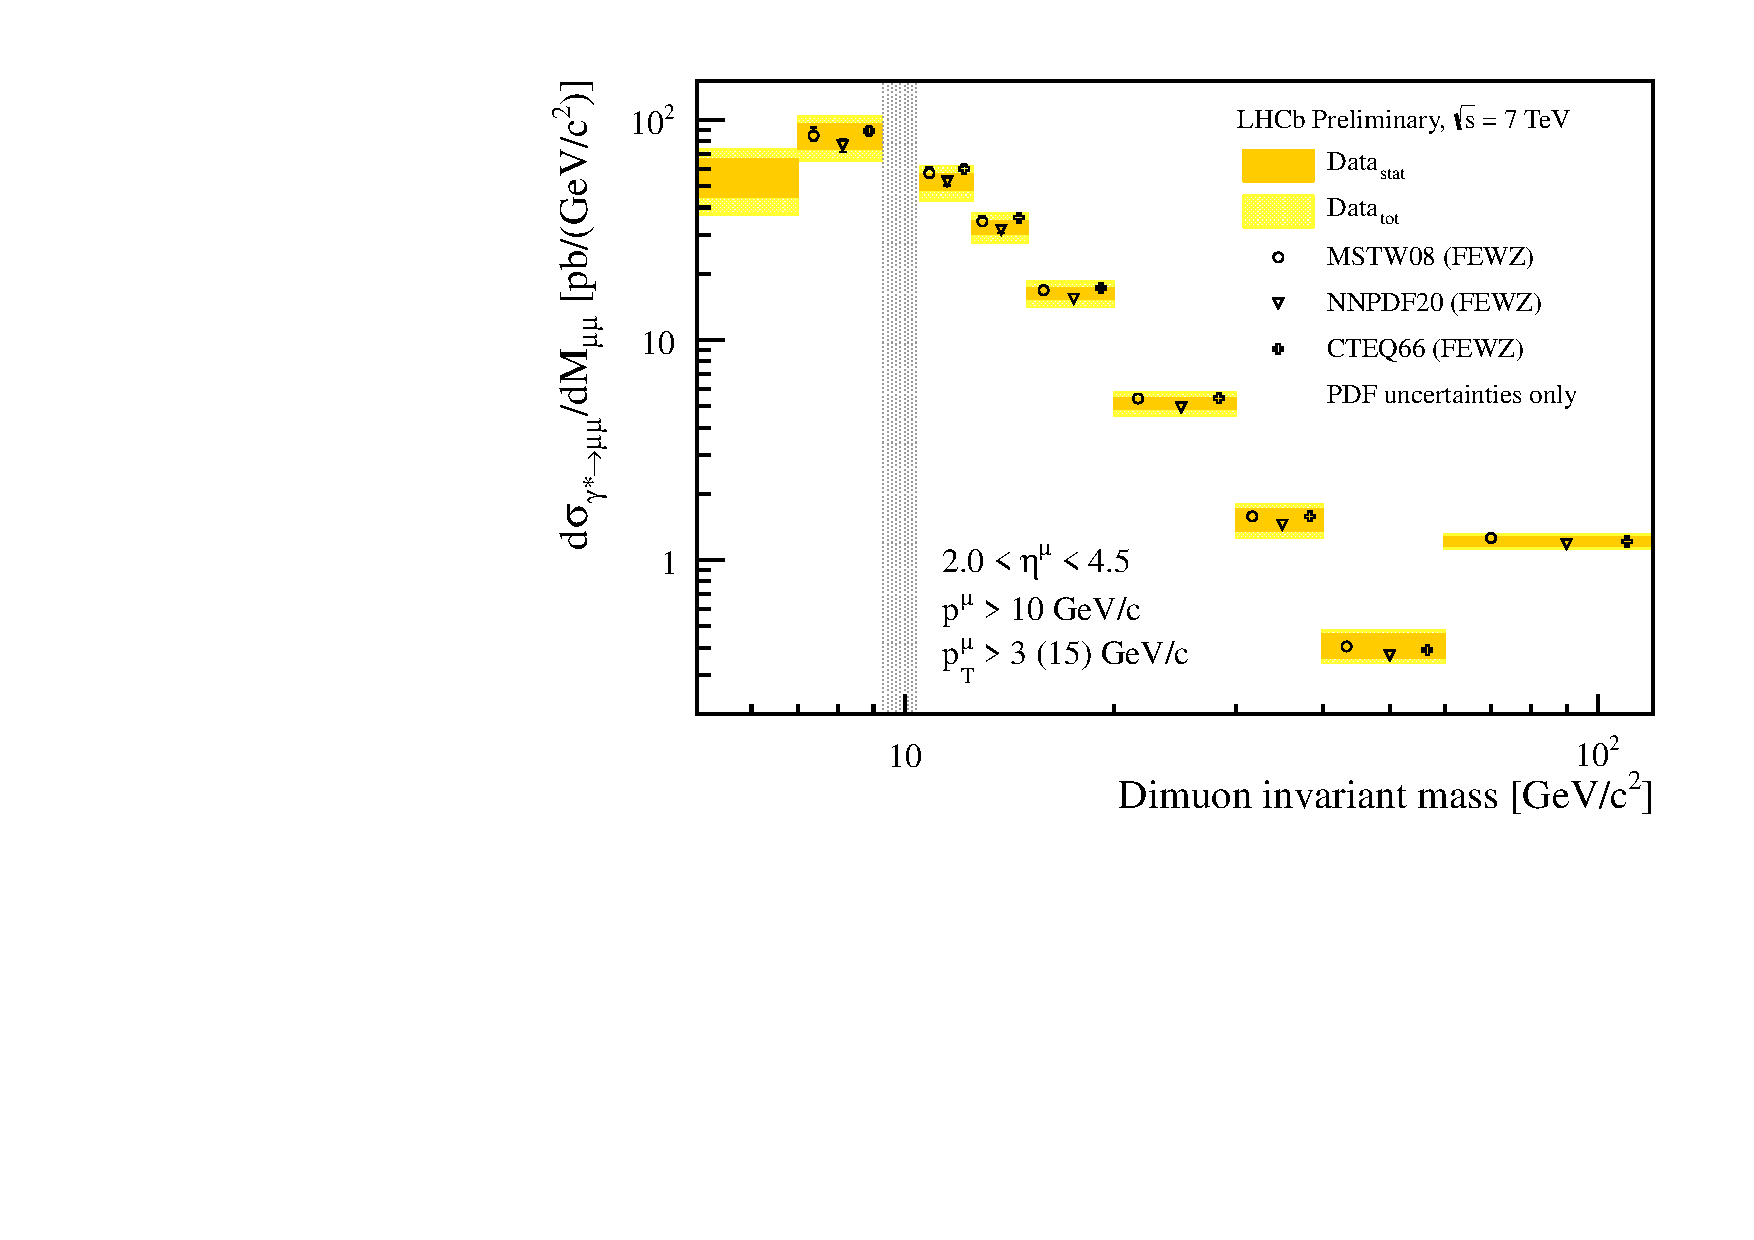
\includegraphics[width=0.5\textwidth]{\main/smallx/fig/CSDYM2.pdf}
\caption{low-mass Drell-Yan invariant mass LHCb from pp, to be replaced by projection plot with appropriate luminosity. could be combined in one plot with W,Z from ATLAS/CMS}
\end{figure}

\begin{figure}[htb]
\centering
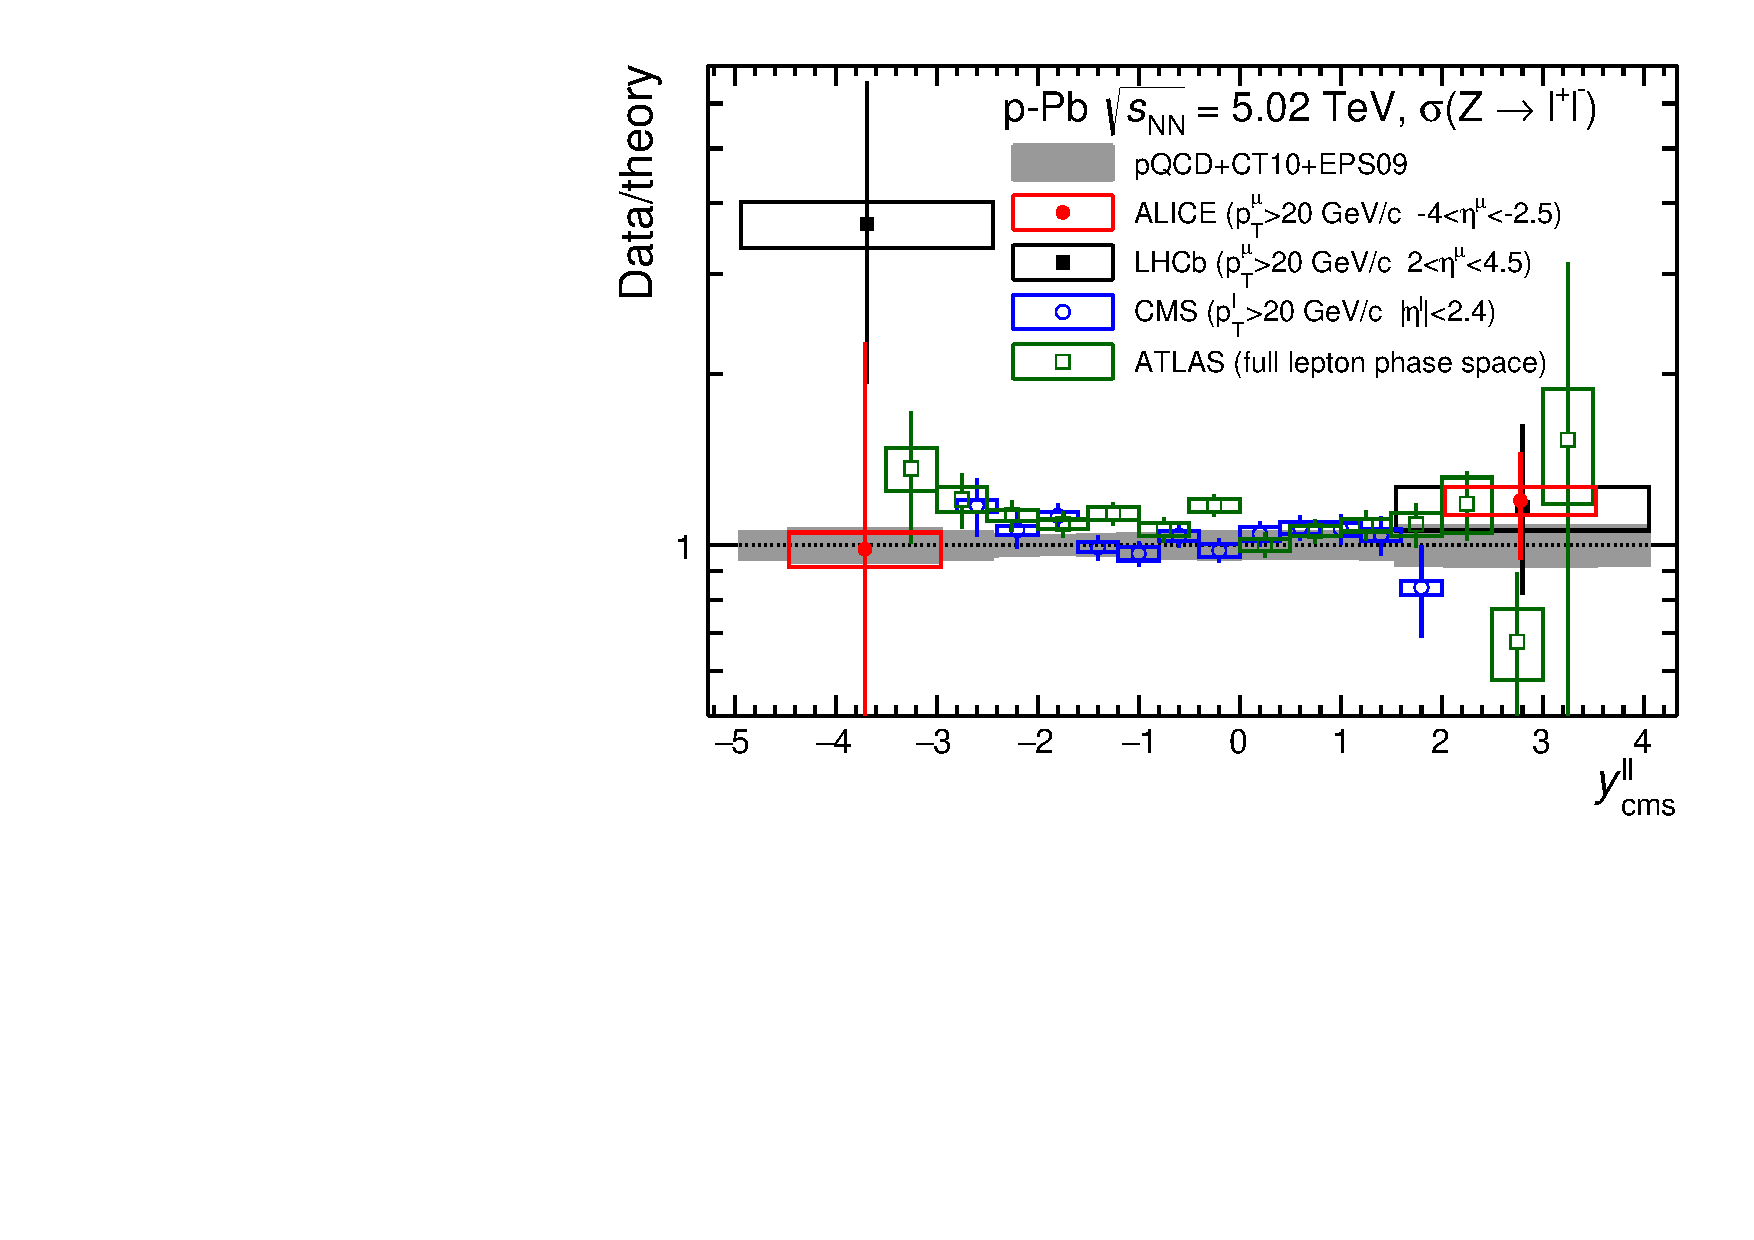
\includegraphics[width=0.5\textwidth]{\main/smallx/fig/placeholder_z_pPb_ALICE.pdf}
\caption{Measured Z boson production cross-section in p-Pb collisions at $\sqrt{s_{\rm NN}} = 5.02$~TeV divided by the theoretical expectations, to be replaced with the expected statistical significance of the Z boson rapidity distribution for p-Pb collisions at $\sqrt{s_{\rm NN}} = 8.8$~TeV in run 3-4 assuming an integrated luminosity of 0.25/pb (0.25/pb) obtained with the proton (Pb ion) going toward the muon spectrometer. In the estimation, a conservative detector efficiency of 70\% is used. The results are compared with the statistical significance of the published data collected in p-Pb collisions in 2013.}
\end{figure}



 ccbar correlations (LHCb)
\begin{figure}
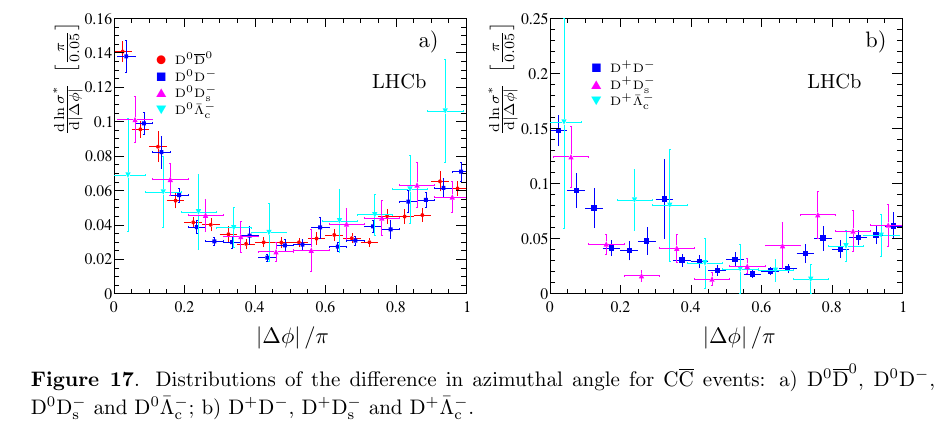
\includegraphics[width=1.0\textwidth]{\main/smallx/fig/placeholderppmeas.png}
\caption{placeholder from pp for ccbar correlations plot from LHCb in pPb}
\end{figure}

\subsubsection{TMD and Low-$x$ phenomena sensitive observables in $c\bar{c}$ and $b\bar{b}$ production }
Editor:  Cyrille Marquet\\
Content: c-cbar and b-bbar correlations: heavy-mesons and dijets \\
Indicative length: 1-2 page
\subsubsection{Fully coherent energy loss effects on different final states}
Editor: Francois Arleo\\
Content: Drell-Yan/photons, E-loss, pt-broadening in pA\\
Indicative length: 1-2 page

The multiple scattering of quarks and gluons traveling in a QCD medium induces the radiation of gluons which carry away some energy of the propagating parton, leading for instance to the jet quenching phenomenon (see Section~\ref{}). Therefore, a key ingredient of any parton energy loss calculation is  the medium-induced gluon spectrum radiated by the fast propagating color charge. It is of course of crucial importance to know the correct parametric dependence of the induced spectrum, which in general depends on the parton properties (in particular its energy and mass) and those of the medium, since it has a direct impact on the phenomenology of particle production in pA and AA collisions. The emission of a gluon radiated by an energetic parton experiencing multiple scattering in a medium takes a typical formation time, $t_f$, which needs to be compared to the length of the medium, $L$.

Over the last few years, it has been realized that in a hard process involving incoming and outgoing energetic color charges (which do not have to be identical) being quasi-collinear in the rest frame of the medium, the associated medium-induced gluon spectrum is dominated by {\it large} gluon formation times, $t_f \gg L$. In this so-called fully coherent (FC) region, the medium-induced radiated energy is similar to the energy loss of an asymptotic charge. In particular it scales as the energy, and thus exceeds at high energy the average parton energy loss in the Landau--Pomeranchuk--Migdal (LPM) regime, $t_f \lesssim L$, for which the energy dependence is at most logarithmic.
%
This different parametric behavior has important consequences on the phenomenology of hadron production in pA collisions. In particular, a model based on the fully coherent induced gluon spectrum was shown to describe accurately the quarkonium suppression observed in pA collisions at all center-of-mass energies, from the SPS fixed-target experiments ($\sqrt{s}\simeq 20$~GeV) to the LHC ($\sqrt{s}=5.02$~TeV and $\sqrt{s}=8.16$~TeV). It is therefore necessary to investigate further the role of fully coherent energy loss on other processes.
%
Because the fully coherent induced gluon spectrum arises from the interference between the emission amplitudes off the initial charge and that off the final state, the effects of FC energy loss are process dependent. Let us review, at a qualitative level, the expected nuclear dependence of different processes which could be measured at the LHC with a high luminosity.

In the absence of color charge in the partonic final state, the energy loss in Drell-Yan (DY) production at leading order is expected to be that of a suddenly decelerated parton, that is, independent of its energy (LPM regime). The effects of parton energy loss in nuclei should therefore play almost no role on DY production in high-energy pA collisions, since $\Delta E / E \to 0$ in the high-energy limit. The inclusive production of DY lepton pairs in pA collisions at the LHC should therefore be free of any parton energy loss effect. As a result, this process might be used advantageously in order to probe possible nuclear PDF effects at small values of $x$, see \eg Fig.~\ref{fig:plotDY} and Ref.~\cite{Arleo:2015qiv} for more details. Assuming a luminosity of ${\cal L}=250$~nb$^{-1}$ and taking the conservative value for the cross section in pPb collisions at $\sqrt{s}=5$~TeV, ${\rm d}\sigma/dy=40$~nb~\cite{Arleo:2015qiv}, the number of forward DY lepton pair, which could be measured by the LHCb experiment is typically $10^4$ per rapidity unit. Also interesting, and accessible with a high luminosity, would be the production of diphotons in pA collisions. This process would be free of energy loss effects, for the same reasons as the DY process, while being sensitive to nPDF in the quark sector, $q\bar{q} \to \gamma\gamma$, and in the gluon sector through the `box diagram', $gg \to \gamma\gamma$.

Note that the energy loss scaling as $E$ (FC regime) would come into play only if {\it another} energetic charged particle is produced in the final-state in association with the virtual photon (or the diphoton), such that the final state carries a global color charge. Such a situation typically occurs in DY$+$jet production in pA collisions. Consider for instance the Compton scattering process, $qg \to q\gamma^\star$. At forward rapidity, an incoming quark from the proton projectile scatters in the medium to produce the final state in a color triplet representation. In this peculiar case of quark to a color triplet final state, one would expect a negative medium-induced gluon spectrum, leading to an energy \emph{gain} (with respect to pp collisions), $\Delta E \propto (-1/2N_c)\times E$. Such an unusual dependence would manifest by a slight \emph{enhancement} of DY+jet production in pA collisions with respect to pp collisions, although a quantitative study would be needed to answer whether this effect could be visible in the experiment. Similarly, should this enhancement be small or negligible, the associate production of a prompt photon with a heavy-quark jet might be sensitive to the nPDF of heavy quarks and gluons, as emphasized in Ref.~\cite{Stavreva:2010mw}. Using $\sigma_{\gamma c} = 1.2\times10^5$~pb in the acceptance of the ALICE calorimeter~\cite{Stavreva:2010mw} leads to $2.4\times10^5$ $\gamma+c$-jet events in pPb collisions at $\sqrt{s}=8.8$~TeV assuming ${\cal L}=2$~pb$^{-1}$.

More pronounced effects of fully coherent energy loss are expected when the final state is in a color octet state, or possibly in higher color representations. An example is the production of a jet pair with not too large transverse momenta (ideally only a few times the saturation scale of the target nucleus). In the case of di-gluon production, the final state can be produced in the 27-plet color representation (with Casimir $C_{27}=8$) that would lead to an average coherent energy loss proportional to $(N_c+C_{27})/2=11/2$, that is almost twice larger that expected if the final state is in a color octet state. Such higher color representations could also be probed in the production of $B_c$ mesons (or in the associate production of a D and a B meson), with a complex final state $c\,\bar{c}\,b\,\bar{b}$. From the number of fitted signal candidates ${\cal N}=10^4$ $B_c$ mesons extracted at LHCb in the semileptonic decay channel in pp collisions at $\sqrt{s}=8$~TeV with ${\cal L}=2$~fb$^{-1}$~\cite{Aaij:2014bva}, the expected $B_c$ rate in the LHCb acceptance using ${\cal L}=0.5$~pb$^{-1}$ in pPb collisions ${\cal L}=0.5$~nb$^{-1}$at the same energy is ${\cal N}=5\times 10^2$ $B_c$ mesons.

\subsection{Constraints on nuclear pdf at the HL-LHC}
\label{sec:nPDFs}
Editors: see subparts\\
Indicative length: 5 pages
\subsubsection{Overview}
Editors: Fred Olness, Aleksander Kusina, Ingo Schienbein, Hannu Paukkunen,   Ilkka Helenius\\
Indicative length: 2 pages \\
Content: summary of 'safe' inputs referring to sub-chapter tables, discussion of their impact and global fit to pseudodata and discussion of theory progress to enlarge 'safe' observables: low-x resummation, NNLO for heavy-quark c,b observables, necessary input assumptions and how to confirm/falsify with measurements
outlook trying to fold in progress to be expected from experiment/theory and also consequences for Initial state description in heavy-ions \\
Figures: summary plots for nPDF with and without reweight of pseudodata


\subsubsection{$W^\pm$/Z Production}

Recent LHC W/Z  vector boson production
data in heavy ion  collisions are quite sensitive to the
heavier flavors (especially the strange PDF), and this complements the
information from fixed-target  neutrino-DIS data.\cite{Kusina:2016fxy}

OUTLINE: sketch current status/uncertainty, short-comings (u/d asymmetry, strange),
and where improvements can be expected. Will try to update the below 
ratio plots for various luminosity assumptions. 


Measurements: 
\begin{enumerate}
\item 
W/Z differential in $dy$ and $dp_T$, [small $p_T$ need to address resummation] 

\item 
$W^\pm/Z$ cross section correlations,

\item 
 W/Z+ heavy quark (access to strange and heavy quark PDFs; pp at LHC, need pA and AA 
as it is likely these can benefit from high luminosity run.
\\
updates from cms\cite{Chatrchyan:2013uja} and atlas\cite{Aad:2014xca}


\end{enumerate}



\begin{figure}[ht]
\centering{} 
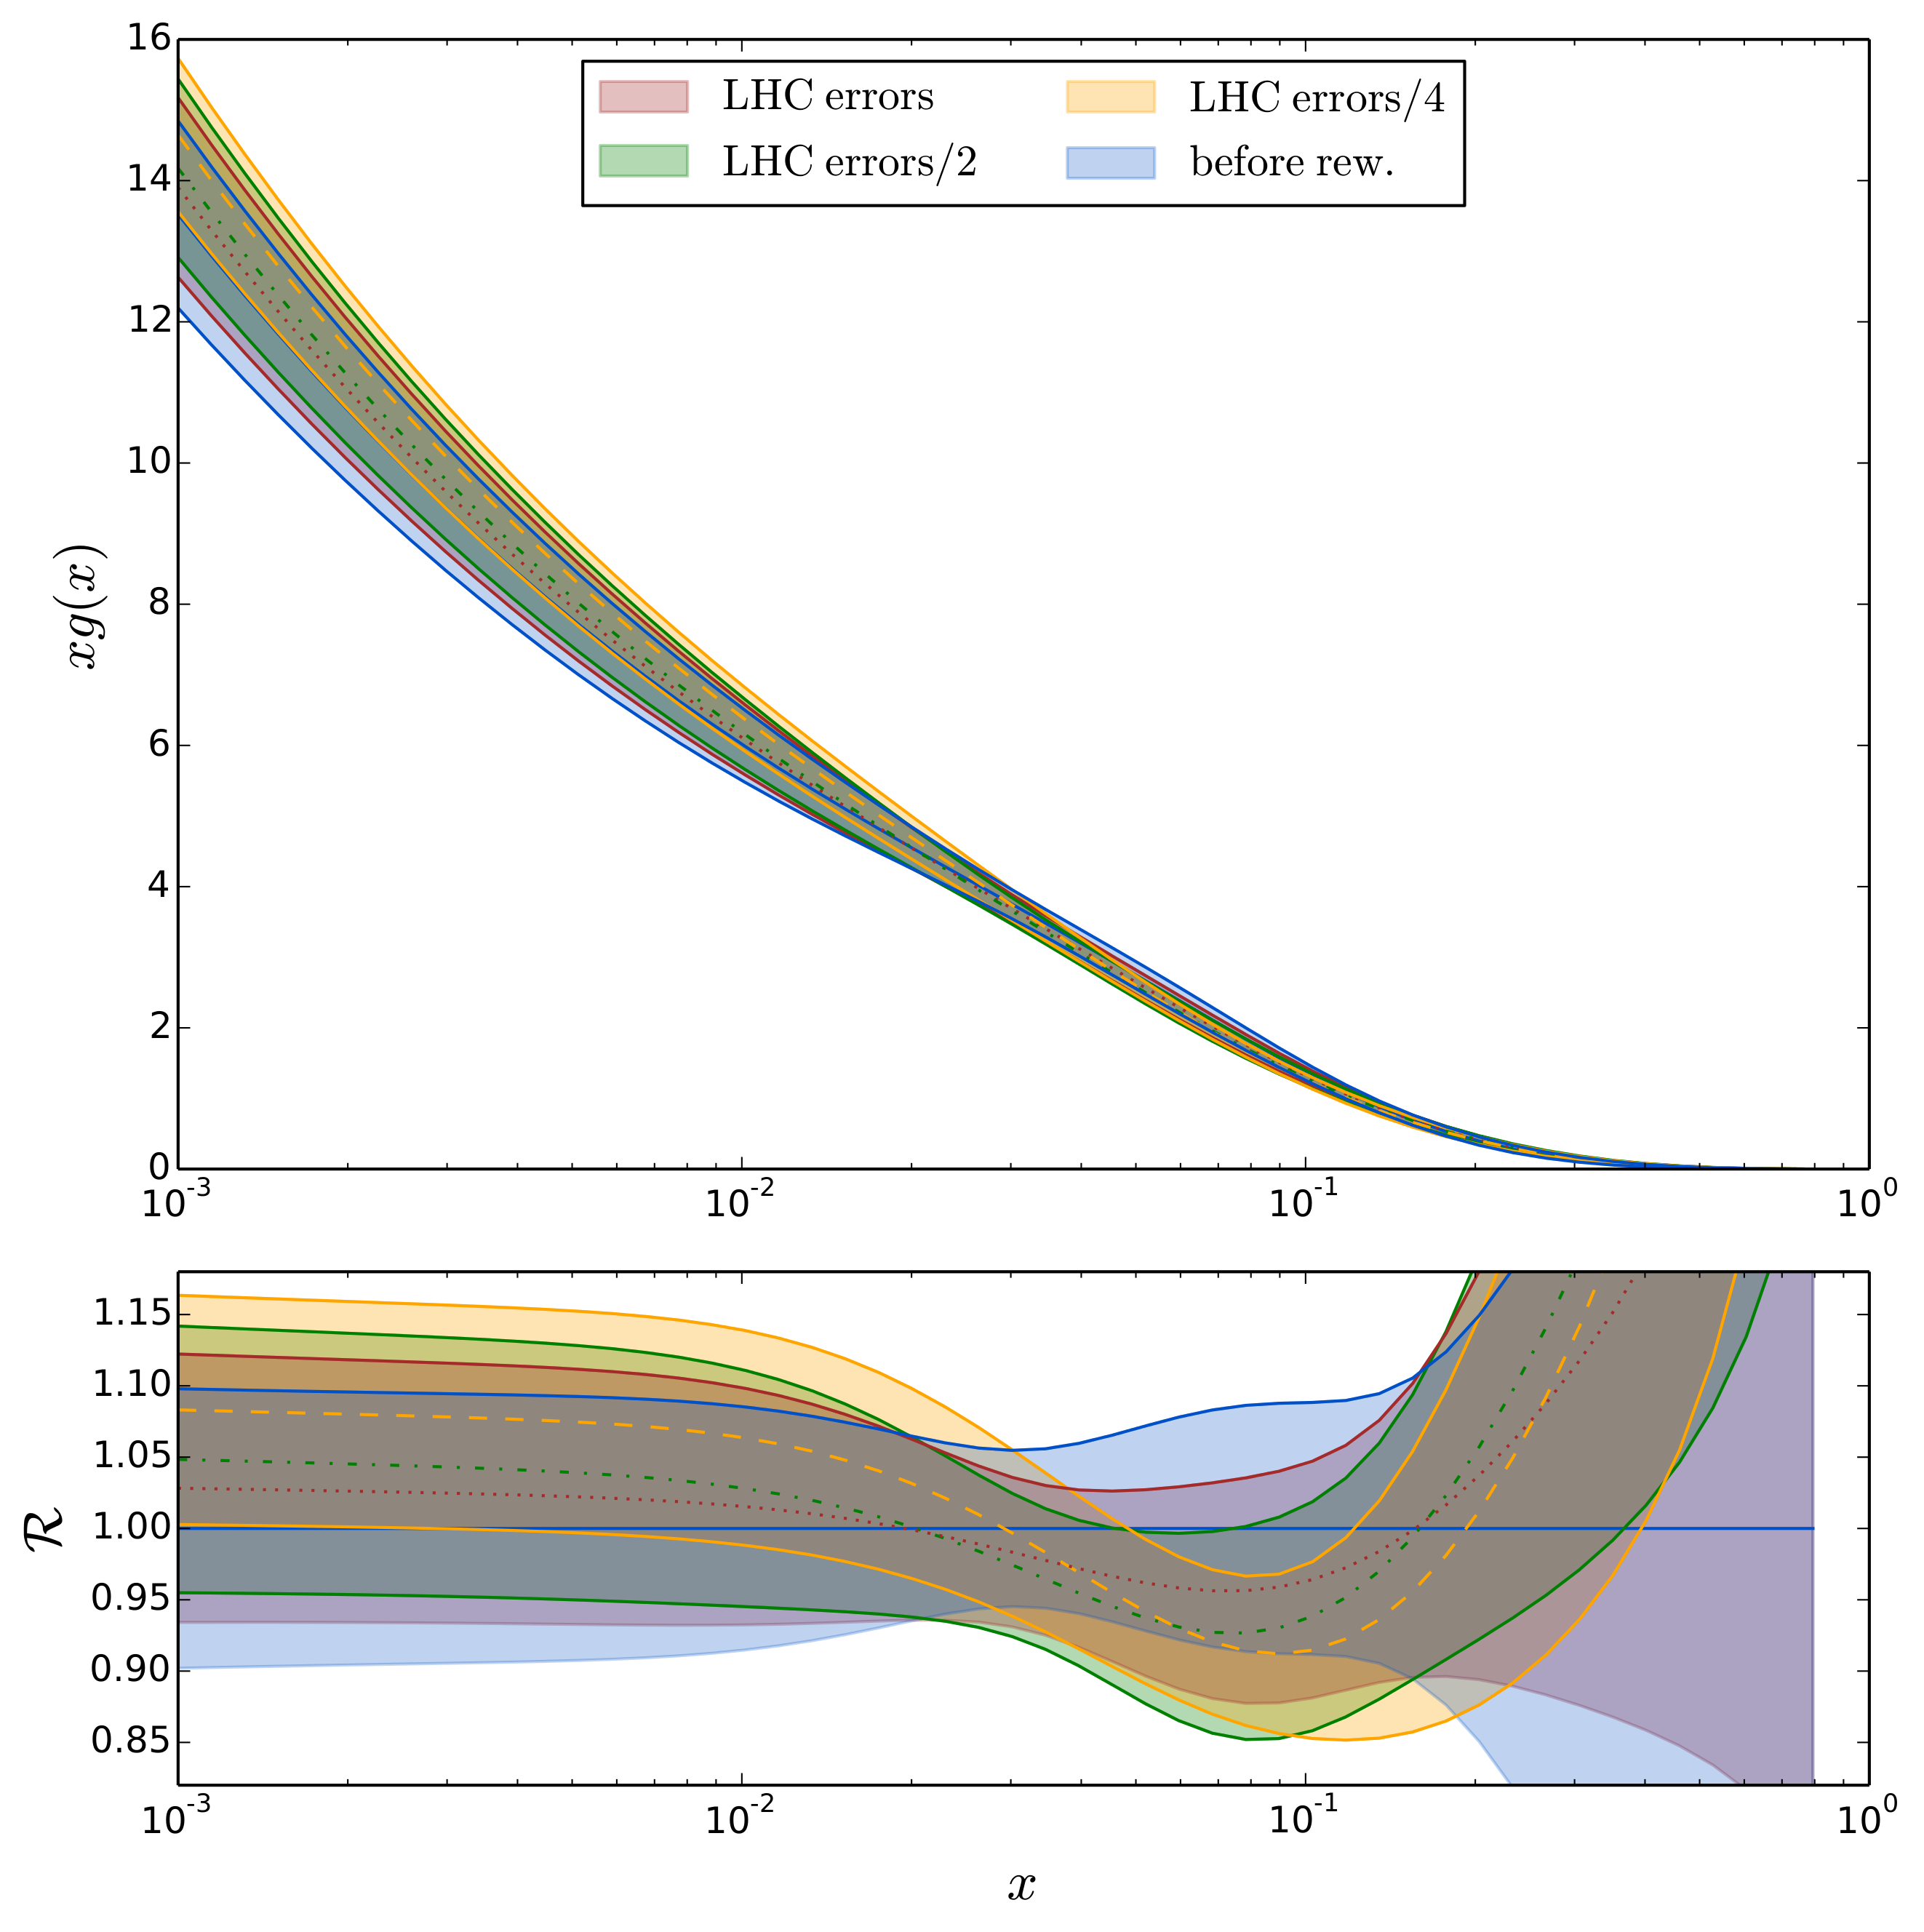
\includegraphics[width=0.30\textwidth]{\main/smallx/fig/sampleLum.png}
\hfil
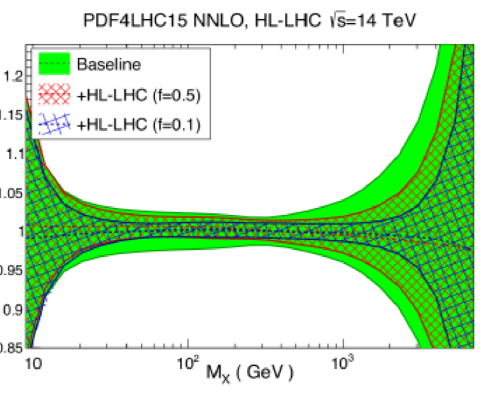
\includegraphics[width=0.30\textwidth]{\main/smallx/fig/pdfTMP2.png}
\caption{
\textcolor{red}{place-holder figures: real ones to be generated}
We display the PDF uncertainty as a function of $x$ 
showing the potential improvement for various luminosity assumptions.
\textcolor{blue}{\it note: for the ratio, we should scale  central value to 1 so 
it looks like standard uncertainty plots; see example right.}
(Fred, Olek, Ingo, ...)}
\end{figure}


\subsubsection{Dijet Production}
Editors: Hannu Paukkunen??? ... \\
Indicative length: 1-2 pages 

\noindent
\textcolor{blue}{note: as nCTEQ does not yet have this implemented,
will need to extrapolate from EPPS16\cite{Eskola:2016oht} for this assessment.}
\\
We suggest (Fred \& Ingo) keeping this separate from UPC 
to keep the $hh$ separate from the effective $h \gamma$ 
(the $\gamma$ includes both direct and resolved contributions) as well as other issues.

\subsubsection{Heavy Quark Production}
Editors: Ingo Schienbein, Aleksander Kusina, Fred Olness ... \\
Indicative length: 1-2 pages 

\begin{enumerate}
\item 
\textbf{Inclusive heavy quark production:} \\
 From the abstract:\cite{Kusina:2018pbp}
{\it We use for the first time experimental data for the inclusive heavy quark
production in proton--lead collisions at the LHC in order to improve
our knowledge of the gluon distribution in nuclei. We first check that the
two most recent global nuclear parton distribution analyses (nCTEQ15
and EPPS16) provide a good overall description of the data, and then use
these data in a PDF reweighing analysis. We find a first clear confirmation
of gluon shadowing at small x. Additionally, it demonstrates that the
inclusion of such heavy-flavour data in a global fit would significantly reduce
the uncertainty on the gluon density down to 
$x \simeq 7 \times 10^{-6}$ while keeping
an agreement with the other data of the global fits. Our study accounts
for the factorisation scale uncertainties which become the largest for the
charm(onium) sector.}

\item 
\textbf{prompt photon-production and diphoton production } \\
{\it ... reminder for Ingo:} ... contrast to above Sec.11.4.4: 
if we compare final states that are i) colored and ii) not colored we can test the idea of energy loss
for the e.g., small-x gluon to identify the source of this effect

\item 
\textbf{higher order corrections} \\
 NNLO heavy quark production (same diagrams as NNLO top), yields improved stability. 
... theory issue ...
challenge: large scale uncertainties. 

\item
\textbf{photon+heavy quark}\cite{Stavreva:2010mw,Stavreva:2012aa}\\
interested in both p+p and p+A: 
Tevatron saw a deviation in charm, but NOT bottom. 
Theoretical issues or intrinsic charm??? or ...
Update to current LHC measurements 

\end{enumerate}


\subsubsection{Top production}
Editors: Hannu Paukkunen and David d'Enterria
Indicative length: 1-2 pages \\

\noindent The $p_{\rm T}$ reach for $t\overline{t}$, and constraints for nPDFs (currently we have this for EPS09, though EPPS16/nCTE15 would be better). Probably lepton+jets channel.
\\
the power to constrain large x gluons vs the heavy quark which is lower x
\\
Czakon et al., Pinning down the large-x gluon with NNLO top-quark pair
                        differential distributions   \cite{Czakon:2016olj}

\subsubsection{UPC dijets}
Editors: Ilkka Helenius\\
Indicative length: 1-2 pages\\
\textcolor{green}{???To be merged with UPC dijet section above by Mark et al. to avoid overlap???}\\
\textcolor{blue}{ ???SUGGESTION??? ... to be discussed (Fred, Ingo) 
Maybe keep the UPC section separate as the initial state is   $\gamma p$ rather than $p p$, and 
then within the UPC can separately address: {\it [example refs cited]}\\ 
i)\textbf{ dijets,} \\
ii) \textbf{heavy quark photo-production }($J/\Psi, D, B ...$)~\cite{Aktas:2005bt} (both inclusive \& in association with jets), \\
iii) \textbf{inclusive prompt photo-production} and also prompt photons accompanied by jets.~\cite{Bussey:2001xg,Chwastowski:2003aw}\\
{\it [look back at the photo-production processes studies at HERA.]}
}

%Figure \ref{fig:UPCdijetNPDF}: Two plots showing the dijet cross section as a function of $x_A$ with ATLAS cuts on jet kinematics and with softer jet cuts that extend the kinematic reach to lower values of $x$ and $Q^2$. In addition to the absolute cross sections also ratios of the cross section with proton and nuclear PDFs are shown and the nuclear PDF uncertainties are compared to the expected statistical uncertainties assuming LHC and HL-LHC luminosities. Also uncertainties arising from photon PDFs are estimated.\\
%Content: The write-up describes briefly the theoretical framework used in the simulations and discusses about optimal kinematical cuts for constraining the nuclear PDFs at small and intermediate values of $x$. Also the relation between the actual $x$ in the nuclear side and the $x_A$ determined from the momenta of reconstructed jets is examined.
\noindent {\bf DIJETS:}
Ultra-peripheral heavy-ion collisions provide an opportunity to study nuclear modifications of the PDFs in clean photon-nucleus interactions. One possible observable is dijet production as suggested in Ref.~\cite{Strikman:2005yv}. Compared to the dijet production in p+Pb collisions the photo-nuclear events have less underlying event activity since multiparton interactions are significantly suppressed. This enables jet reconstruction at lower transverse momenta allowing to study nPDFs at smaller $Q^2$ and $x$ where the current uncertainties are more pronounced. As the virtuality of the photons emitted by the nucleus is negligible, there are two components that needs to be taken into account: the photons may interact as an unresolved particles or the quasi-real photons may fluctuate into a hadronic state described with photon PDFs. The relative contribution of the direct and resolved components depends on the studied kinematics so the uncertainty related to weakly-constrained photon PDFs can be reduced by focusing on the region where direct processes dominate the dijet production.

Here we apply the photoproduction framework recently implemented into the \textsc{Pythia 8} Monte-Carlo event generator \cite{Sjostrand:2014zea}, validated against HERA data \cite{Helenius:2018bai}, to study the potential of the HL-LHC program to constrain nPDFs using photo-nuclear dijets. The relevant part of the photon flux is obtained by integrating the impact-parameter dependent flux from $b_{\mathrm{min}}=2 R_{\mathrm{Pb}} \approx 13.27\Ufm$. We consider two different jet kinematics, one corresponding to the preliminary ATLAS measurement \cite{ATLAS:2017kwa} with $p_{\mathrm{T}}^{\mathrm{lead}}>20\UGeVc$ and $m_{\mathrm{jets}} > 35\UGeV$ and one similar to HERA dijet photoproduction data with $p_{\mathrm{T}}^{\mathrm{lead}}>8\UGeVc$ and $m_{\mathrm{jets}} > 14\UGeV$. In both cases the jets were reconstructed from the generated events using anti-$k_{\mathrm{T}}$ algorithm with $R = 0.4$ implemented in \textsc{FastJet} package \cite{Cacciari:2011ma}. The differential cross sections are shown as a function of $x_A$ (defined from jet momenta as in Ref.~\cite{ATLAS:2017kwa}) in Fig. \ref{fig:UPCdijetNPDF} using \textsc{NNPDF2.3lo} proton PDFs \cite{Ball:2012cx} with and without EPPS16 nuclear modifications \cite{Eskola:2016oht}. The uncertainty bands are derived from EPPS16 error sets and reflects the uncertainties in the current the nPDF analyses which are compared to expected statistical uncertainties of the data in the ratio plots. Also the contributions from direct and resolved processes are separately plotted. Furthermore, results with the default CJKL photon PDFs \cite{Cornet:2002iy} are compared to GRV \cite{Gluck:1991jc} and \textsc{SaSgam} \cite{Schuler:1995fk} analyses to study the underlying photon PDF uncertainty.

As shown in the left panel of Figure~\ref{fig:UPCdijetNPDF}, the contribution from resolved processes becomes dominant around $x_A > 0.02$ for $p_{\mathrm{T}}^{\mathrm{lead}}>20\UGeVc$. This leads to a more pronounced dependence on the photon PDFs in this region, partly hindering the use of the data from this region in a global nPDF analysis. However, at small-$x$ region, where the nPDF uncertainties are currently large and the dijets in p+Pb do not provide additional constraints, the direct processes dominate the dijet production and the dependence on the photon PDFs is negligible. The dijet cross sections fall off rapidly at small-$x_A$ region which increases the expected statistical uncertainty limiting the small-$x_A$ reach of the observable. With the integrated luminosity of the heavy-ion program of the LHC ($L=1\Unb^{-1}$) and jet kinematics of the ATLAS preliminary study the expected statistical uncertainties become significant at $x_A \lesssim 2 \cdot 10^{-3}$. The increased luminosity and $\sqrt{s_{\mathrm{NN}}}$ of the HL-LHC increase the potential small-$x_A$ reach only slightly but in the region where nPDF constraints are currently sparse. An effective way to extend the small-$x_A$ reach is to consider jets with lower $p_{\mathrm{T}}$ as demonstrated in the right panel of Figure~\ref{fig:UPCdijetNPDF}. With a cut of $p_{\mathrm{T}}^{\mathrm{lead}}>8\UGeVc$ and integrated luminosity of the HL-LHC ($L=13\Unb^{-1}$) it is possible to obtain nPDF constraints down to $x_A \approx 10^{-4}$.  Also, the small-$x$ nPDF uncertainties are more pronounced with lower $p_{\mathrm{T}}^{\mathrm{lead}}$-cut since the nuclei are probed at smaller scales. In principle a baseline measurement for UPC dijets with a proton target could be performed in p+Pb collisions to reduce the theoretical and experimental uncertainties but since the energy spectrum of photons is correlated with the impact parameter the kinematics would not be fully comparable. However, $x_A$ distributions normalized with the integrated cross section would still be sensitive to the shape of the cross section and could be used as an alternative observable in nPDF fits to reduce theoretical and experimental uncertainties.

\begin{figure}
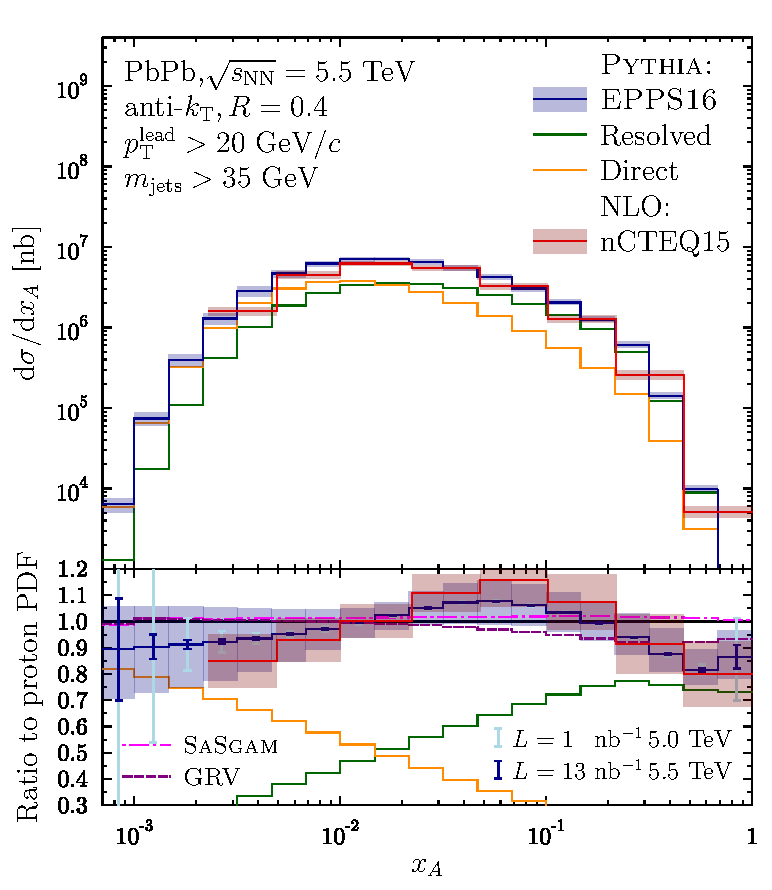
\includegraphics[width=0.49\textwidth]{\main/smallx/fig/plotxA_ATLAS.pdf}
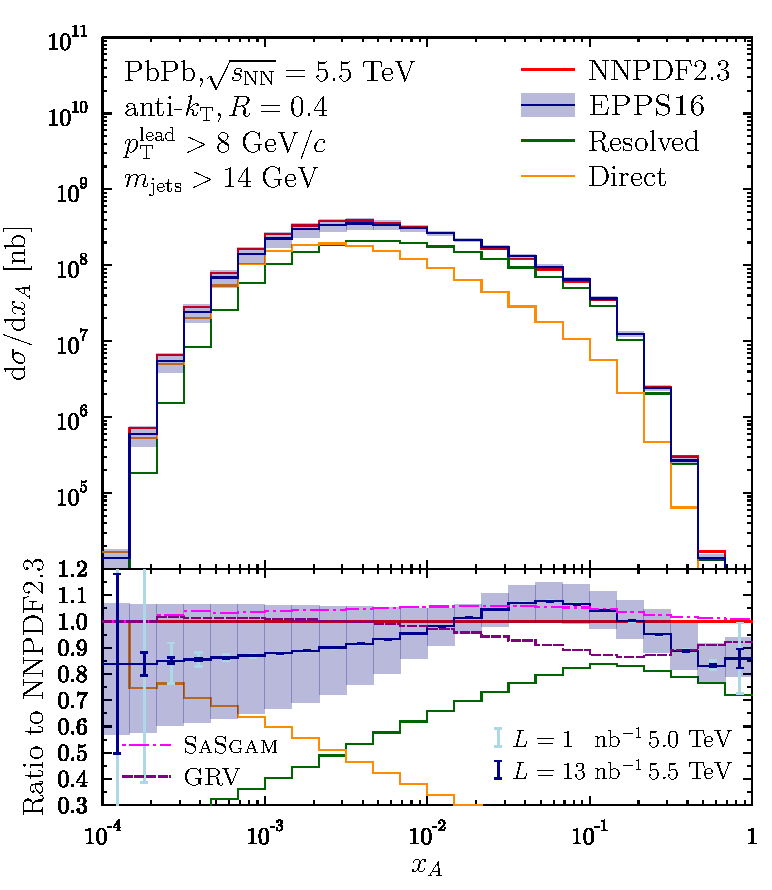
\includegraphics[width=0.49\textwidth]{\main/smallx/fig/plotxA_pTlow.pdf}
\caption{Photo-nuclear dijet cross-sections in ultra-peripheral Pb+Pb collisions with leading jet $p_{\mathrm{T}}$ cut of $20\UGeVc$ (left) and $8\UGeVc$ (right). Results with EPPS16 nuclear modification (blue) and with proton PDFs only (red) are shown separately as also the contributions from resolved (green) and direct (orange) photons. Ratio plots show also results with different photon PDF sets and the expected statistical uncertainties corresponding to the LHC (light blue) and the HL-LHC (dark blue) luminosities.}
\label{fig:UPCdijetNPDF}
\end{figure}



\subsection{Perspectives with lighter ions}
To be confirmed, lumis to be given in the accelerator part \\
Editors: Nestor Armesto, Fred Olness \\
Indicative length: 1-2 pages \\

Lighter ions, with the possibility to achieve large integrated luminosities in modest running times, see Sect. {\bf ????}, offer several interesting opportunities for the study of the initial stage of ion collisions, for small-$x$ physics and for the determination of nuclear parton densities, see Subsection \ref{sec:smallxIntro}.

First, concerning nPDFs, it should be noted that due to the scarcity of nuclear data, a PDF fit for a single nucleus is impossible as discussed in Subsection \ref{sec:smallxIntro}. The different groups \cite{deFlorian:2011fp,Kovarik:2015cma,Eskola:2016oht}  have adopted different strategies but, generically, they give the parameters in the initial condition to be fitted a dependence on the nuclear mass number. Such dependence acquires different functional forms and, therefore, it constitutes part of the parametrisation bias in the nPDF set. Data on lighter nuclei may help to constrain such parametrisations, see the discussions for UPCs and pA collisions in Subsection \ref{sec:nPDFs}.

On the other hand, the impact parameter dependence of nPDFs is linked to their dependence on nuclear size. Several models exist (see e.g. \cite{Emelyanov:1998phs,Ferreiro:2008wc}), and even less model-dependent approaches like the EPS09s analysis \cite{Helenius:2012wd} where the dependence on nuclear size was used to constrain the impact parameter dependence. Besides, first-principle calculations (named Gribov inelastic shadowing) relate diffraction in electron-proton collisions with nuclear shadowing. This has been used to predict nuclear shadowing \cite{Frankfurt:2011cs,Armesto:2003fi}, including its nuclear size and impact parameter dependence. While such relation is exact for deuteron, its extension to larger nuclei has some degree of model-dependency. Lighter ions are the ideal place to test the nuclear size dependence without resourcing to centrality selection, whose relation with impact parameter is doomed to be as problematic - at least - as found in pA collisions.

Lighter ions also offer large luminosities that are important for several aspects:
\begin{itemize}
\item Data on beauty mesons and bottomonium in pA can be used to constrain nPDFs \cite{Kusina:2017gkz} better than their charm counterparts, because of the larger scale given by the mass and by the opportunity that they are less affected by collective effects. But they demand large statistics that can be achieved with lighter ions.
\item Larger luminosities will benefit measurements in pA for observables with large scales, like high-mass DY or dijets, for precise determination of nPDFs.
\item UPCs and photon-photon studies \cite{Baltz:2007kq} will be greatly benefited in spite of the $Z^{2(4)}$ factor for the photon luminosities that can be overcompensated by the larger nucleon-nucleon luminosity .
\item Larger luminosities can also benefit small-$x$ forward observables that, like dijets \cite{Dainese:2016gch}, aim to reach quite large transverse momenta.
\end{itemize}

Lighter ions offer a bridge between small systems and PbPb without requiring centrality selection that is problematic both in pp, pA and peripheral AA. 
Besides, in the framework of saturation models \cite{Gelis:2010nm} that aim to describe collective effects in small systems without requiring final state interactions (see e.g. \cite{Kovner:2016wsq} and references therein), the extension from the proton to the nuclear case in phenomenological realizations  is done by a simple rescaling of the squared saturation momentum $Q_s^2\propto A^{1/3}$. And the centrality dependence is assumed to be proportional to the nuclear profile, which leads to strong problems in the nuclear periphery where a dilute situation is restored. Lighter ions offer a check of our ideas on the
nuclear size versus energy leading
the density that determines saturation, and the use of minimum bias observables
instead of centrality-sliced ones that
would greatly simplify the phenomenology.

To conclude, lighter ions offer several pros and cons for initial stage studies. The main con is the fact that theory calculations usually assume the limit of scattering of a dilute projectile (proton) on a dense target (nucleus). Lighter ions are further from this limit. On the other hand, they offer: (i) a bridge between small and large systems without resourcing to
centrality selection that would be useful for constraining the nuclear wave function, the
collision dynamics and the interpretation of collectivity;
(ii) the possibility of larger luminosities for UPCs, forward observables,$\dots$,
for nPDFs determination and small-x studies; and (iii)
a more affordable setup for microscopic calculations of corrections.

\end{document}